\section{Basic Usage}

The package is based on \TikZ{} and the main command should be used in a \texttt{tikzpicture} or -- as shown in some of the examples -- with \verb+\tikz+.

\subsection{The shirts}
 The package provides a number of shirts for the bear, \bearwearkey{long sleeves} and \bearwearkey{round neckline} are the defaults:
 \begin{tcblisting}{righthand width=6cm}
 \tikz\bearwear % default
    [long sleeves,
     round neckline];
 \tikz\bearwear
   [t-shirt];
 \tikz\bearwear
   [muscle shirt];

 \tikz\bearwear
   [v-neckline];
 \tikz\bearwear
   [t-shirt,v-neckline];
 \tikz\bearwear
   [muscle shirt,v-neckline];
  \end{tcblisting}

 \subsection{Dressing the bear}

 To dress the bear with the shirt, simply add the \verb+\bear+ command from the \bearwearkey{tikzlings-bears} package.

 \begin{tcblisting}{before=\nopagebreak}
 \tikz{\bear;\bearwear[v-neckline];}
 \tikz{\bear;\bearwear[muscle shirt];}
  \end{tcblisting}

 \subsection{Coloring the shirts}

 The body and the arms of the shirts can be colored. They are three basic keys: \bearwearkey{leftarm}, \bearwearkey{rightarm} and \bearwearkey{body}, and two meta keys: \bearwearkey{arms} and \bearwearkey{shirt}.

 \begin{tcblisting}{tikz lower}
  \bear;
  \bearwear
    [v-neckline,
     leftarm=red,
     rightarm=green,
     body=blue];
 \end{tcblisting}
 \begin{tcblisting}{tikz lower}
  \bear;
  \bearwear[arms=green];
 \end{tcblisting}
 \begin{tcblisting}{tikz lower}
  \bear;
  \bearwear
    [shirt=
      {shade,
       top color=blue,
       bottom color=red}];
 \end{tcblisting}


 Basically every option that would make sense in a \verb+\fill+  is allowed here.
 Patterns e.g. would work too:

 \begin{tcblisting}{tikz lower}
   \bear;
   \bearwear
     [v-neckline,
      shirt  =
        {pattern=
          horizontal lines light blue}];
 \end{tcblisting}


 \subsection{Additional patterns}

 As seen in the last example patterns can be added instead of colors, but sometimes it makes sense to
 add them on top to preserve a background color. For this the package provides special \texttt{pattern} keys:\\
 \bearwearkey{leftarm pattern}, \bearwearkey{rightarm pattern}, \bearwearkey{arms pattern},
 \bearwearkey{body pattern}, \bearwearkey{shirt pattern},

 \begin{tcblisting}{tikz lower}
  \bear;
  \bearwear
     [v-neckline,
      shirt=red,
      body pattern =
       {pattern=
         {Stars[points=6,
          radius=0.5mm,distance=1.5mm]},
        pattern color=yellow}];
 \end{tcblisting}



 \subsection{Decorations}

 The \lstinline|deco| keys add their value to a \texttt{path picture} key. This can be used to place emblems or use graphics as pattern. To help with the placement two coordinates are
 predefined: \bearwearkey{bearheart} and \bearwearkey{beartummy}.

 \begin{tcblisting}{tikz lower}
   \bear;
   \bearwear[shirt deco =
    {\fill[red] (beartummy) circle (1pt);
     \fill[red] (bearheart) circle (1pt);}
     ]
\end{tcblisting}

\begin{tcblisting}{tikz lower}
  \bear;
  \bearwear[shirt deco =
    {\node at (beartummy) 
     {
\includegraphics[width=5cm]
       {tartan3}};}]
\end{tcblisting}    

\begin{tcblisting}{tikz lower}
  \bear;
  \bearwear[body deco=
    {\node at ([yshift=-1mm]bearheart) 
      {
\includegraphics[width=0.3cm]
        {flag}};}];
\end{tcblisting}    

\begin{tcblisting}{tikz lower}
  \bear;
  \bearwear[
     shirt=Beige!80!black,
     body deco=
      {\node at ([yshift=-1mm]bearheart) 
       {
\includegraphics[width=0.5cm]
         {latex-project-logo}};}];
\end{tcblisting}

\begin{tcblisting}{tikz lower}
  \bear;
  \bearwear[
     shirt=HotPink,
     body deco=
      {\path  (bearheart)--++(0,-3mm)
        pic{hippo};}];
 \end{tcblisting}


\begin{tcblisting}{tikz lower}
  \bear;
  \bearwear[
    arms= DeepSkyBlue,
    body deco =
     {\node at ([yshift=-2mm]beartummy) 
       {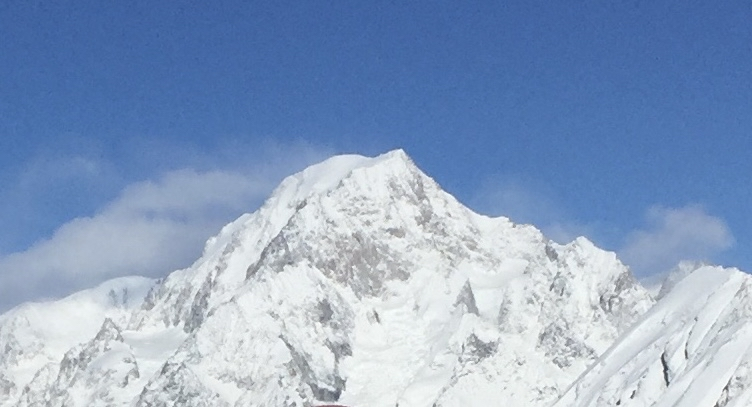
\includegraphics[width=4cm]
         {montblanc}};
      \node[text=white,
           font=\tiny\sffamily] 
        at ([yshift=1.95mm]beartummy) 
        {{Mont Blanc}};
     }]
 \end{tcblisting}
 
 \subsection{Scaling}
 
 Scaling works as expected, but don't forget that nodes in \TikZ{} normally don't scale if you don't use the \lstinline|transform shape| key:
 
 \begin{tcblisting}{tikz lower,before=\nopagebreak,}
  \begin{scope}[scale=1.5]
  \bear;
  \bearwear[
    arms= DeepSkyBlue,
    body deco =
     {\node at ([yshift=-2mm]beartummy)
       {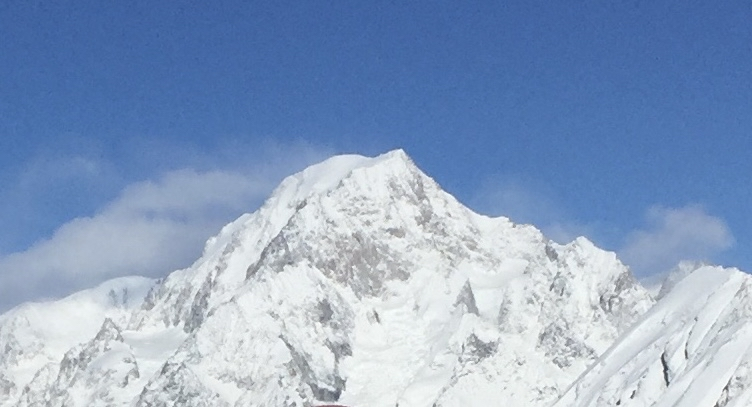
\includegraphics[width=4cm]
         {montblanc}};
      \node[text=white,
           font=\tiny\sffamily]
        at ([yshift=2mm]beartummy)
        {{Mont Blanc}};
     }]
   \end{scope}  
 \end{tcblisting}
 
 \section{The brains behind \bearwearlogo{}}
 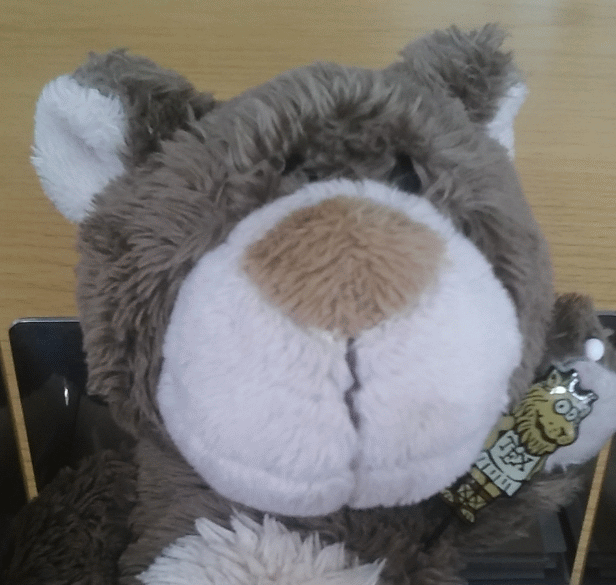
\includegraphics[width=3cm]{baer}
 \begin{description}
 \item[Ulrike]
  Bär, your decision to create \bearwearlogo{} has come as a surprise to many. Did you expect this?
  \item[Bär] Quite true, Ulrike. I am better known as an outdoor type
  and the fashionistas didn't reckon with me at all.
 \item[Ulrike] So, why did you take this step?
 \item[Bär] There were quite a few reasons -- most importantly
 my deeply felt desire to bring more justice to the world.
 Look at the wonderful world of \TikZ ducks fashion, and even Marmots have come
 far in the area of refinement. Why should \TikZ bears be left behind?
 \item[Ulrike] You are also concerned with the more momentous issues of our day.
 \item[Bär] Correct! My fashion line is the first ever to have practically
 no negative influence on our environment. Manufacture and transportation
 are ecologically neutral. In fact it's the first time in the
 history of world economy that goods are produced without
 the use of raw materials.
 \item[Ulrike] You claim that \bearwearlogo{} will have a global impact.
 \item[Bär] Yes, the issue of globalization is one which has been interesting
  me for a long time. \bearwearlogo{} caters for the needs of \TikZ bears all
  over the world. There is the Longshirt Line for those who live near the poles,
  t-shirts for those in temperate regions and even a Muscle Shirt Line for the
  bears of Australia.
 \item[Ulrike] How about individuality?
 \item[Bär] I am particularly proud that \bearwearlogo{} enables every single
 bear to create his own personal shirt -- free of the dictates of the modern
 Brummells. He may use my suggestions but he need not do so.
 \item[Ulrike] Will you be seen wearing your own creations?
 \item[Bär] Well Ulrike, I am afraid this is not very likely.
 I have got this most beautiful fur and I'd hate to  cover it with artifical
 patterns -- no matter how ravishing.
 \item[Ulrike] One last question: what impulse got you moving towards
 \bearwearlogo{}?
 \item[Bär] The death of Karl Lagerfeld. Someone had to fill the void.
 \end{description}
